\PassOptionsToPackage{dvipsnames}{xcolor}
\input{settings} % add packages, settings, and declarations in settings.tex

\title{ECE 411 \\ Homework 7 - Test Plan}
\date{12/4/2020\\Version 1.0}
\author{Smart Bird Feeder \\Stevie Nicks and the Xaybanha Zhous - Group 9\\Stevie Taylor, Zeming Zhou, Nick Short, Calvin Xaybanha}

\begin{document}
	\vspace{0.3\baselineskip} % Whitespace 
	\maketitle
	\newpage
	
	\tableofcontents
	\newpage
	
	\lhead{} 
	\rhead{ECE 411 - 12/4/2020 \\ Stevie Nicks and the Xaybanha Zhous \\ Homework 7 - Test Plan} 
	\cfoot{\thepage\ of \pageref{LastPage}}
	
	\section{INTRODUCTION}
	\subsection{This Document}
	\newpage
	\section{REFERENCE DOCUMENTS}
	\subsection{Industry Standards}
	\input{references.tex}
	\subsection{Design Documentation}	
	
\begin{minipage}[c]{\textwidth}
	\centering	
	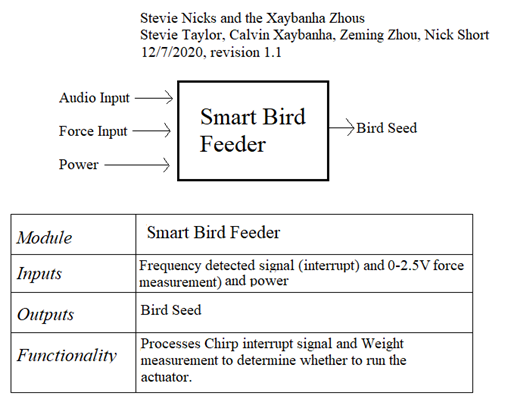
\includegraphics[width=\textwidth]{high_level.png}
\end{minipage}

\bigskip
	\newpage
	\section{OVERVIEW}
	\subsection{Operational Description}
	The objective is to use a microcontroller to only release seed if the microphone is activated above a threshold frequency and the weight sensor feels a weight less than the threshold, above which is assumed to be a crow or squirrel.

The device will use a processing module to automatically dispense bird feed when a small bird is "detected". This is coded using a microcontroller to output a PWM which activates the servo to release seed based on the inputs sensed by the microphone activate with a chirp above the frequency threshold and a strain gauge sensor with a voltage related to the weight on the sensor below the weight threshold.

	\subsection{Definition of Terminology}
	\input{terminology.tex}
	\subsection{Computational Methods}
	Force is in volts.

Frequency is in kilohertz.

	\newpage
	\section{PRETEST PREPARATION}
	\subsection{Test Equipment}
	\input{test_equipment.tex}
	\subsection{Test Setup and Calibration}
	\input{test_setup.tex}
	\newpage
	\section{SYSTEM TESTS}
	\subsection{Functional Tests}
	\subsubsection{Power Switch and Indicator}
	\subsubsection{Servo Test}
	\input{test_case_1.tex} 
	\newpage
	\subsubsection{Mass Sensor Test}
	\input{test_case_2.tex} 
	\subsection{7 Day Stability}
	\subsection{Vibration of Bird Landing on Device Stability Tests}
	
\end{document}



